\section{Findings}

These engagements resulted in the conception and evolution of a design of an IVR system, which would be integrated into PC's existing infrastructure to support the domestic workers in interacting with the digital platform without requiring them to use new physical devices. 

\subsection{Initial Requirements Gathering}

\subsection{Design Iteration 1}

\begin{figure*}
  \centering
  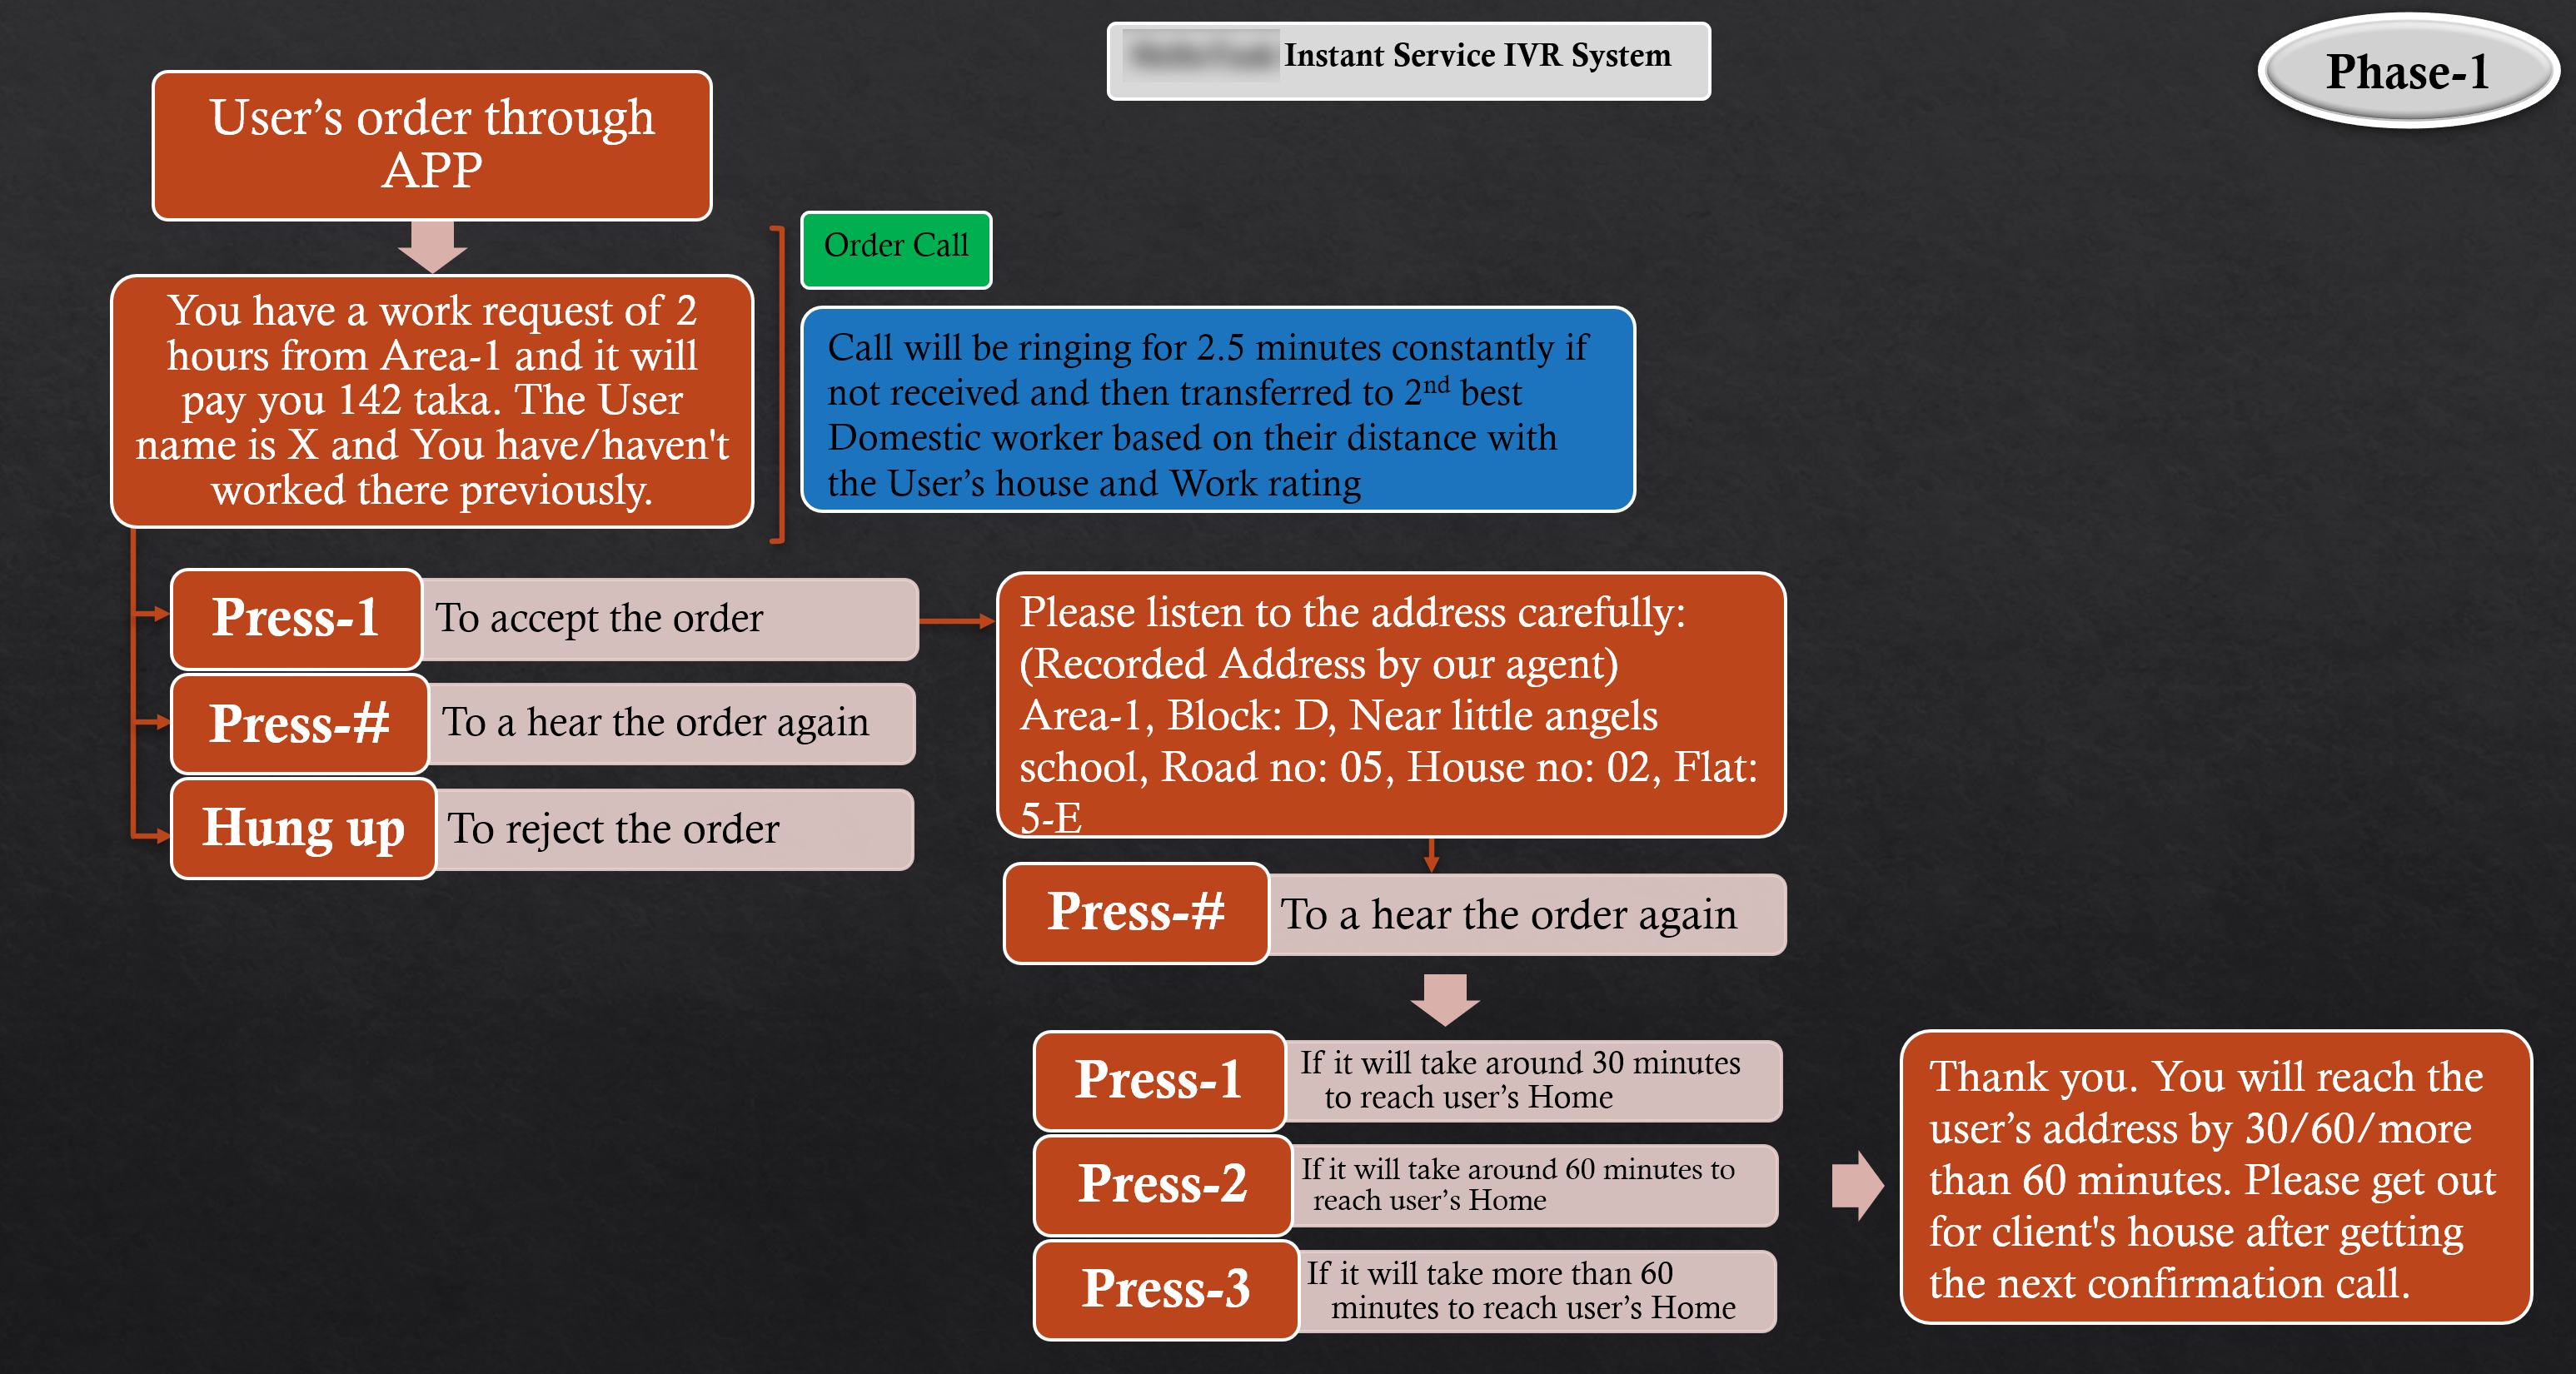
\includegraphics[width=\columnwidth]{images/ivr_01_ordercall.png}
  \caption{PC2's initial PowerPoint design of the `order calls' stage, which would dial domestic workers with information about a job, and ask them for an estimated time of arrival.}~\label{fig:OrderCalls}
\end{figure*}

\begin{figure*}
  \centering
  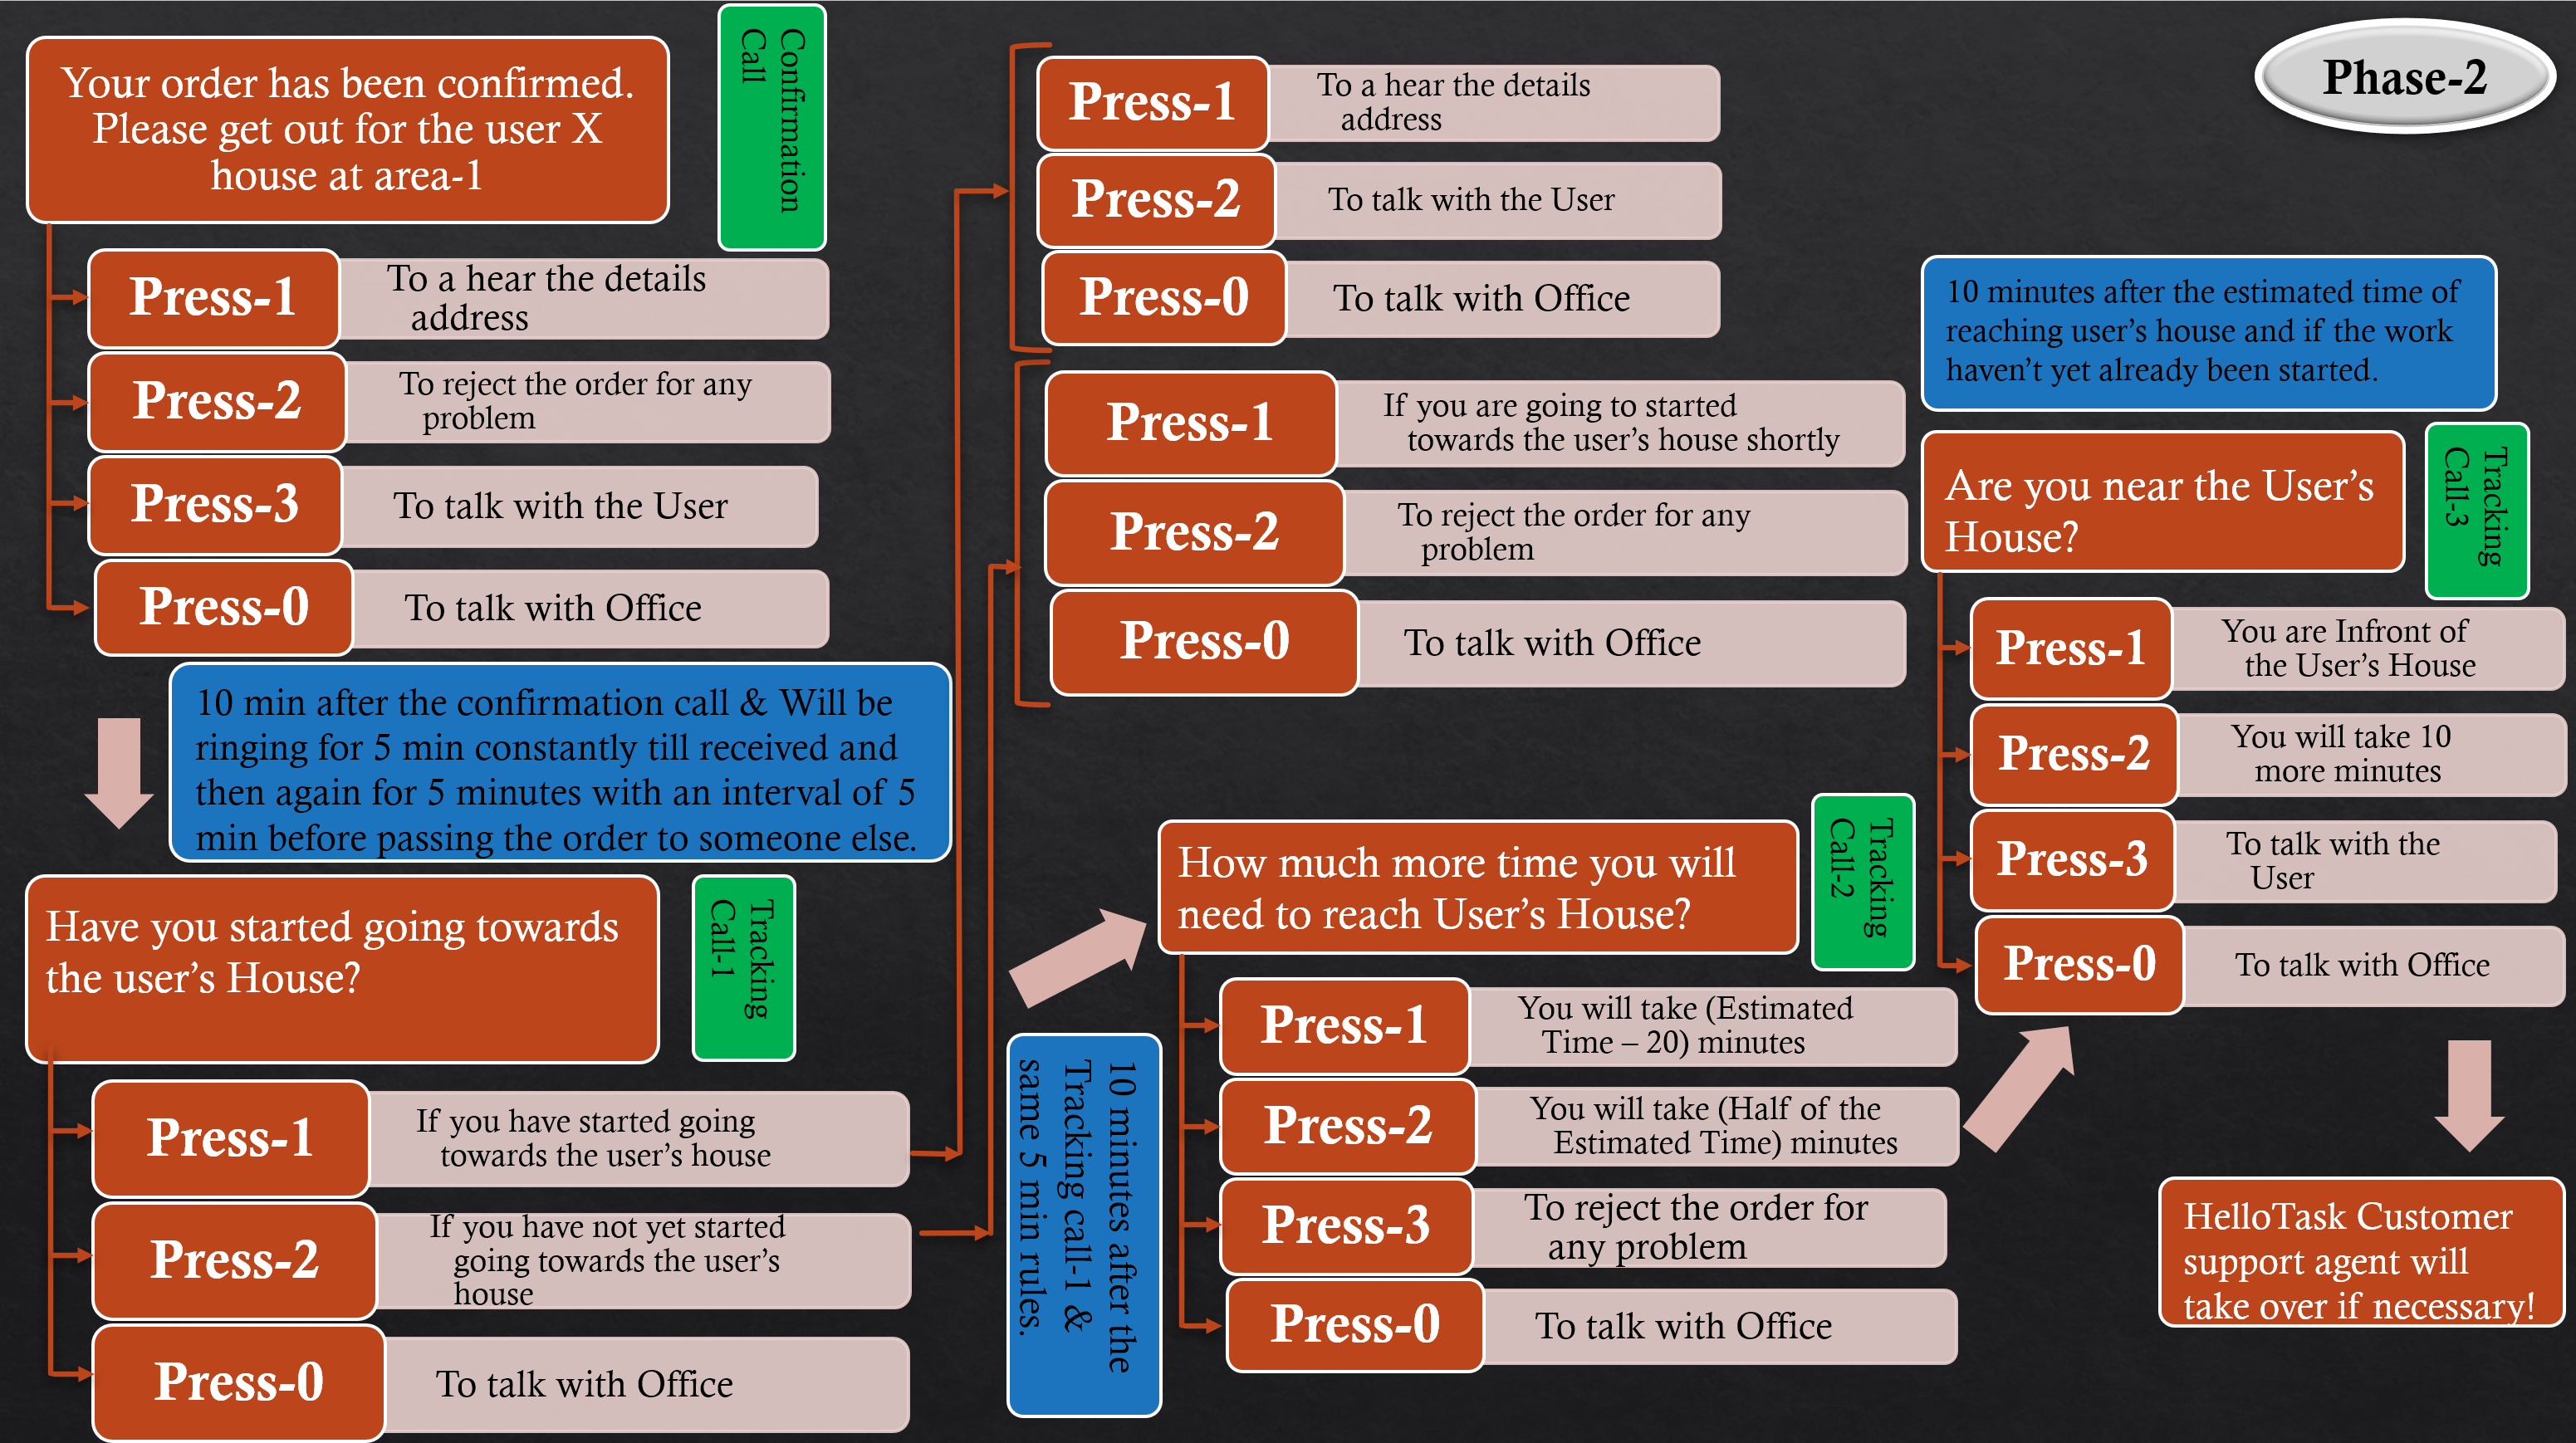
\includegraphics[width=\columnwidth]{images/ivr_01_tracking.png}
  \caption{The initial design of the `tracking calls' stage, describing a confirmation call and three `tracking' calls to be made to domestic workers, intended to check on their progress as they travel to their client's house.}~\label{fig:TrackingCalls}
\end{figure*}

\begin{figure*}
  \centering
  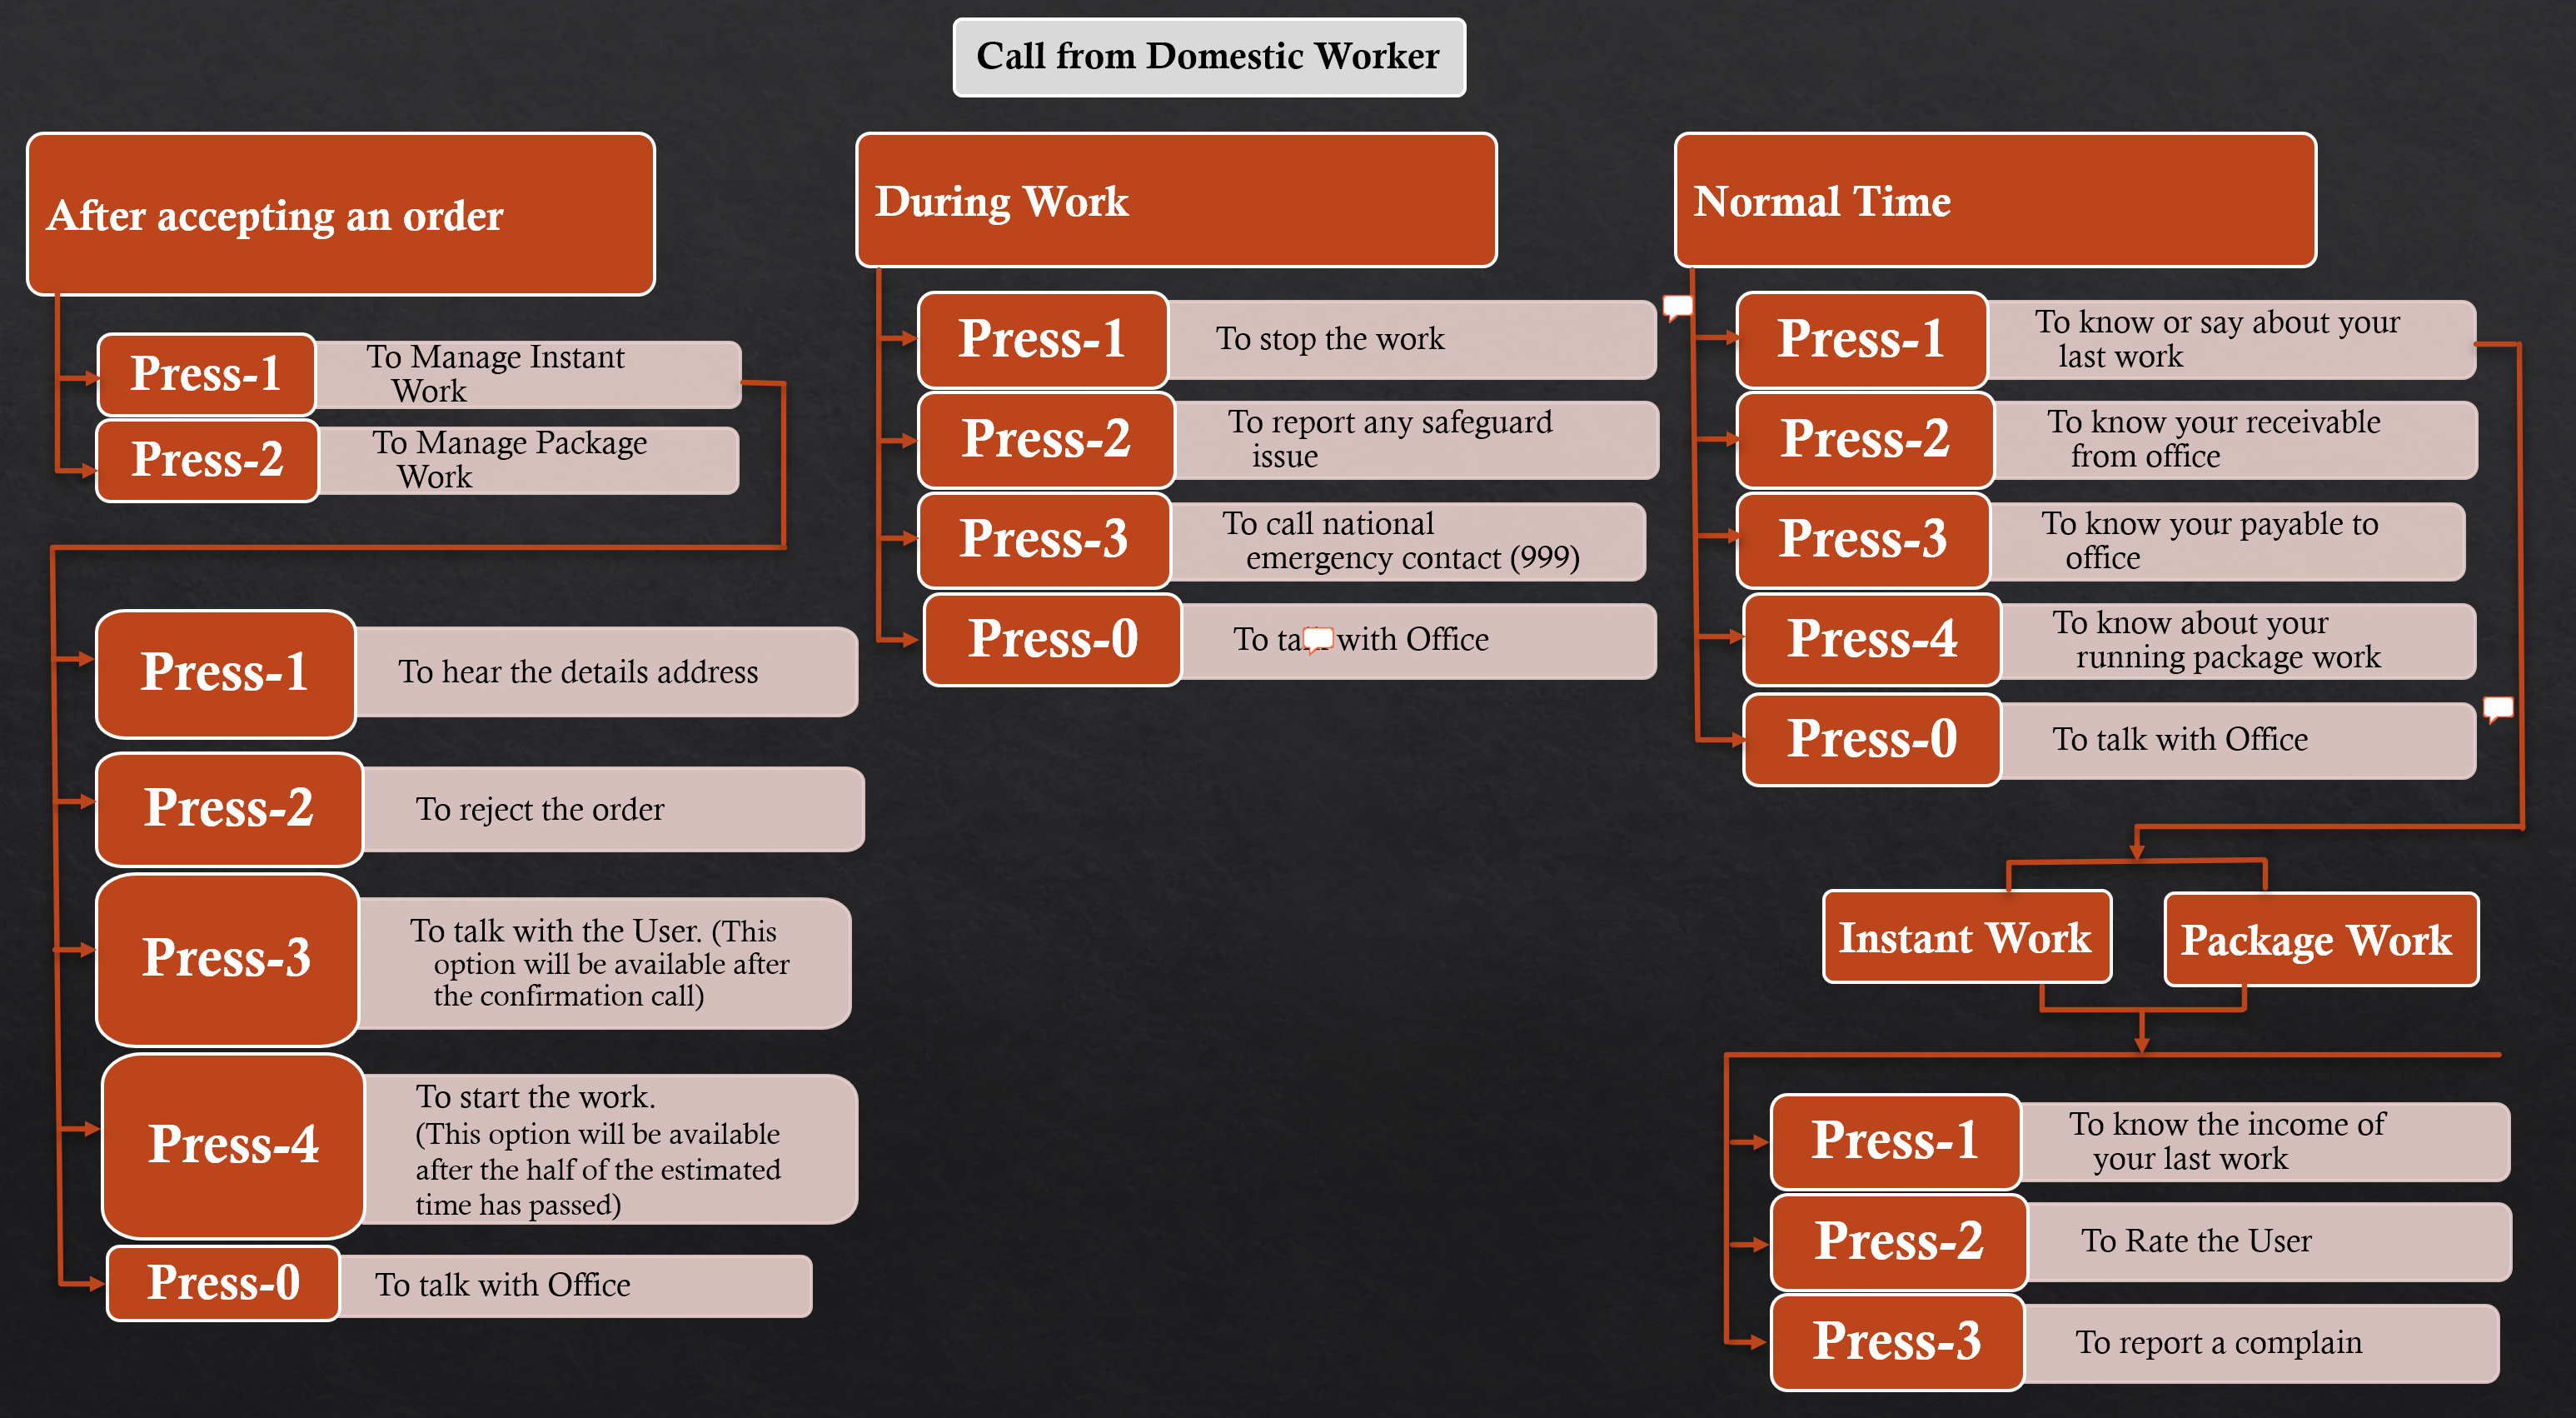
\includegraphics[width=\columnwidth]{images/ivr_01_inbound.png}
  \caption{The initial design of the way the IVR system would handle inbound calls from domestic workers. The menu presented to the workers varies depending on the worker's current work state within the system.}~\label{fig:InboundCalls}
\end{figure*}

Following our first meeting, PC2 shared with us an initial design of the system in Microsoft PowerPoint. This design detailed the `IVR flow': the menus, information and options available to the domestic workers as they interact with the system over the phone. The PowerPoint consisted of three slides, each describing a different type of phone call that the system would make or receive:

\begin{itemize}
    \item The first slide (Fig \ref{fig:OrderCalls}) described the `order calls' stage: outbound calls made by the system to the workers, offering them a job and giving them some basic information about the client's location. If they accepted, the worker would then be asked to give an estimation of how long it would take for them to reach the client (an `ETA', with options of 30 minutes, one hour, or longer than one hour).
    \item The second slide (Fig \ref{fig:TrackingCalls}) detailed the `confirmation call' and three `tracking calls' which would the worker would receive from the system. The tracking calls ask the worker for updated ETA, as well as giving them the option to call PC's office or the client. These tracking calls would  be made at intervals of ten minutes after the worker received the confirmation call. 
    \item The third slide (Fig \ref{fig:InboundCalls}) described how inbound calls made by the domestic worker dialling into the system would be handled. The design offered one of three different menus to the worker depending on their current `state': if they were on their way to a client's house they would get options to hear the address details, dial the client, dial the PC office, or log the work as having started; if they were at a house on a job they would get the option of logging the work as having finished, reporting safeguarding issues, contact the emergency services or call the office; or if they didn't currently have a job assigned the could leave a rating for their last client, get information about their earnings, or contact the office.
\end{itemize}

In response to this design, we responded with a document containing a number of questions and concerns we had about the design to be addressed in the next meeting. As well as technical points of interest (e.g. `\textit{What happens if a worker's call disconnects before they give their ETA?}'), these included queries about the underlying system (e.g. `\textit{How are workers currently/previously chosen?}'; `\textit{Do the workers' ratings of the clients get used? If so, how?}'; `\textit{What's the reason for calling the domestic workers before confirming the job?}'; `\textit{How long can a worker expect to wait for the confirmation call?}'). We also highlighted three major concerns: that the tracking calls don't make allowances for distinguishing between actual travel time and when workers estimate they will arrive (`\textit{The estimated time might not be the same as travel time---the worker might have to finish house work, or organise childcare before leaving the home}'); that the frequent tracking calls are likely to be intrusive (`\textit{It’s also possible that workers will stop answering these tracking calls---being called every few minutes is likely to be annoying if they are travelling/finishing up other tasks.}'); and that the third slide's reliance on dynamic `states' may prevent the workers from being able to easily and reliably memorise the interface (`\textit{May be easier to present the same options each time (even if redundant/non-functional) for the sake of consistency, so that the user knows exactly what the options will be every time they call. This would probably also be simpler to develop and less prone to bugs.}') 



\subsection{Design Iteration 2}

\subsection{Wizard of Oz Prototype}

